\newpage
\section{Asintoti}

\subsection{Asintoto orizzontale}
\begin{definition}[Asintoto orizzontale]
Data una $f: A \to \mathbb{R}$, un $a \in \mathbb{R}$. Se esiste $\lim\limits_{x\to x_0}f(x) = l \in \mathbb{R}$ (finito) si dice che $f$ ha un \textbf{asintoto orizzontale} di equazione $y = l$ per x che tende a $\pm\infty$.
\end{definition}
\begin{example}
Prendiamo $f(x) = e^x$ con $f:\mathbb{R}\to \mathbb{R}$.
\end{example}
\begin{wrapfigure}[7]{l}{7cm}
    \vspace{-5pt}
    \centering
    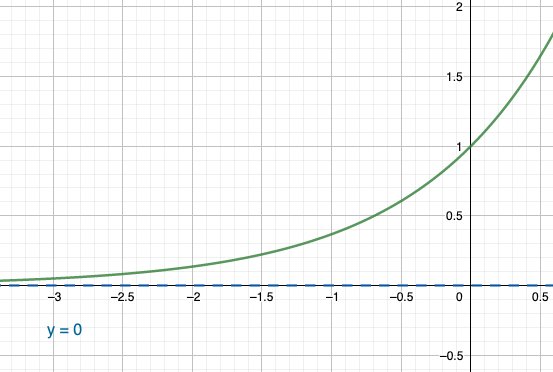
\includegraphics[width=5.5cm]{images/asintoto-esponenziale.png}
    \caption{Asintoto orizzontale di $e^x$}
\end{wrapfigure}

Andiamo come prima cosa a calcolare il limite: $\lim\limits_{x\to -\infty}f(x) = 0$.
Possiamo così vedere che $f$ ha un asintoto orizzontale di equazione $y=0$ per $x\to -\infty$. \\\\
Come possiamo notare nell'immagine a fianco (asintoto segnato dalla linea blu in basso).\\\\\\\\\\

\begin{example}
Facciamo un altro esempio prendendo questa volta $f(x) = \arctan(x)$ con $f: \mathbb{R}\to \mathbb{R}$
\end{example}
\begin{wrapfigure}[9]{r}{7.5cm}
    \vspace{-5pt}
    \centering
    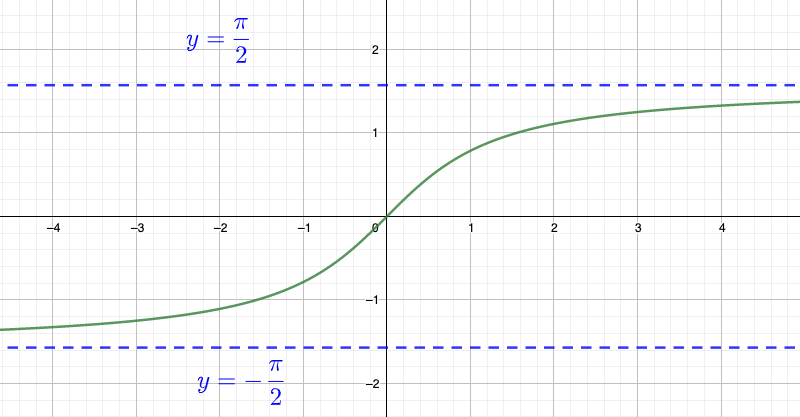
\includegraphics[width=5.5cm]{images/asintoto-arctan.png}
    \caption{Asintoto orizzontale di $\arctan(x)$}
\end{wrapfigure}

Anche qui compre prima cosa calcoliamo il limite sia vero $+\infty$ che verso $-\infty$ della funzione:\\ $\lim\limits_{x \to +\infty}\arctan(x) = \frac{\pi}{2}$
$\lim\limits_{x \to -\infty}\arctan(x) = -\frac{\pi}{2}$\\\\
Vediamo dunque due asintoti con equazioni $y=\frac{\pi}{2}$ e $y=-\frac{\pi}{2}$ rispettivamente con $x\to +\infty$ e $x\to -\infty$.
Possiamo vedere i due asintoti nell'immagine a fianco (rette in blu).\\

\subsection{Asintoto verticale}
\begin{definition}[Asintoto verticale]
Dato un $A \subset \mathbb{R}$, $x_0\in Acc(A)$, $x_0 \in \mathbb{R}$, una $f:A\to \mathbb{R}$. Se $f$ diverge per $x$ che tende a $x_0$ da destra o da sinistra (o da entrambe le parti) si dice che f ha un \textbf{asintoto verticale} di equazione $x=x_0$.
\end{definition}

\begin{example}
Prendiamo la funzione $f(x) = \frac{1}{x}$ definita come $f: \mathbb{R} \setminus \{0\} \to \mathbb{R}$.
\end{example}
\begin{wrapfigure}[9]{r}{7.5cm}
    \vspace{-10pt}
    \centering
    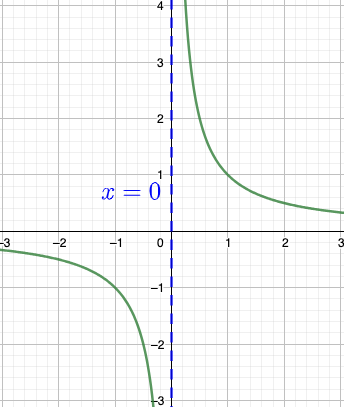
\includegraphics[width=3cm]{images/asintoto-verticale-1.png}
    \caption{Asintoto verticale di $\frac{1}{x}$}
\end{wrapfigure}

Andiamo a calcolare nel punto di discontinuità, che è lo 0, il limite sia da destra che da sinistra:\\\\
$\lim\limits_{x\to 0^+}\frac{1}{x} = +\infty$, $\lim\limits_{x\to 0^-}\frac{1}{x} = -\infty$.\\\\
Vediamo dunque la $f$ ha un asintoto verticale di equazione $x=0$. Possiamo vedere l'asintoto nell'immagine a fianco (asintoto verticale segnato in blu).\\

\begin{observation}
Una funzione al massimo ha 2 asintoti orizzontali (uno a $+\infty$ ed uno a $-\infty$) ma può anche avere $\infty$ asintoti verticali, come nel caso di $f(x) = \tan(x)$ che ha $\infty$ asintoti verticali.
\end{observation}

\subsection{Asintoto obliquo}
\begin{definition}[Asintoto obliquo]
    Data una $f:(a, +\infty) \to \mathbb{R}$. Se esiste $\lim\limits_{x\to +\infty}\frac{f(x)}{x} = m$ con $m \in \mathbb{R}$ e $m\neq 0$, e se esiste anche $\lim\limits_{x\to +\infty}f(x) - mx = q$ con $q \in \mathbb{R}$ allora si dice che $f$ ha un \textbf{asintoto obliquo} di equazione $y = mx + q$ per $x\to +\infty$. Lo stesso vale con $x \to -\infty$.
\end{definition}

\begin{example}
Facciamo un esempio di calcolo dei asintoto obliquo con $f(x) = \frac{2x^2 + 3x +2}{x-5}$.\\
$\lim\limits_{x\to +\infty}\frac{f(x)}{x} = \frac{2x^2 + 3x +2}{x^2-5x} = 2$, quindi $m=2$\\
$\lim\limits_{x\to +\infty}f(x) - mx = \frac{2x^2 + 3x +2}{x-5} - 2x = \lim\limits_{x\to +\infty}\frac{2x^2 + 3x +2 - 2x(x-5)}{x-5} = \lim\limits_{x\to +\infty} \frac{3x + 2 + 10x}{x-5} = \lim\limits_{x\to +\infty}\frac{13x + 2}{x-5} = 13$\\\\
Abbiamo dunque che esiste un asintoto obliquo di equazione $y=2x +13$ per $x\to +\infty$
\end{example}

\begin{observation}
Una funzione può avere al massimo 2 asintoti obliqui (uno a $+\infty$ ed uno a $-\infty$). Inoltre non può avere contemporaneamente un asintoto orizzontale ed uno obliquo "dalla stessa parte".
\end{observation}

\begin{example}
Prendiamo $f(x) = 3x + 5\log(x)$ definita come $f: (0,+\infty) \to \mathbb{R}$. Proviamo ora a calcolare l'asintoto obliquo.\\\\
$\lim\limits_{x\to +\infty}\frac{f(x)}{x} = \lim\limits_{x\to +\infty} \frac{3x + 5\log(x)}{x} = 3 + \lim\limits_{x\to +\infty}\frac{5\log(x)}{x} = 3 + 0 = 3$ quindi $m=3$.\\
$\lim\limits_{x\to +\infty}f(x) - mx = \lim\limits_{x\to +\infty} 3x + 5\log(x) -3x = 5\log(x) = +\infty$.\\\\
Visto che la $q$ non torna un numero finito vediamo che questa funzione non ha asintoto obliquo.
\end{example}